%======   Template created by Jonathan Blair  ========
%=====================================================

%=====================================================
%============ Controls ===============================
%=====================================================

%\documentclass[12pt,letterpaper,onecolumn]{article}
%\documentclass[11pt,letterpaper,onecolumn]{article}
%\documentclass[10pt,letterpaper,onecolumn]{article}
\documentclass[12pt,letterpaper,twocolumn]{article}
%\documentclass[11pt,letterpaper,twocolumn]{article}
%\documentclass[10pt,letterpaper,twocolumn]{article}


\usepackage{amsmath}
\usepackage{graphics}
\usepackage{graphicx} %more modern version of graphics
%\graphicspath{{path-to-folder-containing-necessary-graphics}{other folder as necessary}}


%=====================================================
%============ \begin{document} =======================
%=====================================================

\begin{document}

%=====================================================
%============ Title ==================================
%=====================================================

\title{Investigating the current running through a npn BJT transistor}
%\title{\Large\bf Larger, Bolded Title}

%=====================================================
%============ Author =================================
%=====================================================
\author{
 Garik Livingston and Lily Nguyen \\*
  \\*
 PHY 353L Modern Laboratory \\*
 Department of Physics \\*
 The University of Texas at Austin \\*
 Austin, TX 78712, USA
}
\date{February 11, 2025}

%\address{The University of Texas, Austin, Texas, 78712}

\maketitle

%=====================================================
%============ Abstract ===============================
%=====================================================

\begin{abstract}
	In this experiment we varied the voltage supplied to the base of a npn BJT transistor, and measured the current running through the collector to form a data set which we fitted to the Ebbers-Moll equation.
	From this fit we calculated the thermal voltage ($V_T$) and saturation current ($I_s$). Both these paramaters have strong temperature dependence and from our fit we determined an experimental value for the boltzman constant of $k = 1.378 \times 10^{-23} \pm 8.4 \times 10^{-26} \frac{J}{K}$ for the silicon transistor and a value of k = $5.6 \times 10^{-23}\pm 4.000 \times 10^{-24} \frac{J}{K}$ for the germanium transistor. 
	We also determined an experimental value for the band gap of the transistors with a $E_g = 1.48 \pm 0.012eV$ for silicon and  $E_g = 0.158 \pm 0.003 eV$ for germanium.
	
\end{abstract}

%=====================================================
%============ Body of the article ====================
%=====================================================

%=====================================================
%============ Section ================================

\section{Introduction}

\subsection{Physics Motivation}

The npn Bipolar Transistor (BJT) is a device made of two n doped semiconductor regions called the collector and emitter sandwiched between a p doped base region. 

%Broad physics motivation should be discussed briefly but
%meaningfully. Basic phenomena should be
%explained (or referred to) and
%prediction for experimental results clearly
%stated. Here and throughout the report appropriate
%references should be included~\cite{book, article}.

\subsection{Historical context}

%You may want to relate what you are doing to first or previous
%work on this topic. Since you are doing an experimental work,
%the context should be on the experimental technique. For example,
%you may say that this was first done in a such and such way
%but later it was discovered
%that one can also do it another way. Your technique may be
%related to the first or none of the above.


%=====================================================
%============ Section ================================

\section{Theoretical background}

Provide some more theoretical details for your measurements.
Give formulas and references which provide a specific theoretical
context for your measurements.


%=====================================================
%============ Section ================================

\section{Experimental setup}


\subsection{Apparatus}

Ideas behind the particular technique should be briefly
discussed. Enclose references. Sketches, pictures, and
suitable schematics should be included and explained
concisely. All major components of the system should be
mentioned and their role clearly motivated. This section
is not simply a list of components and it is not an
instruction manual. 


%=====================================================
%============ Importing pictures  ====================
%=====================================================

\subsection{Data Collection}



%Data taking procedures should be described and various modes of
%data collection explained. Calibration procedures and
%relevant plots and numerical tables should be included.
%State clearly what measurements were taken for the final
%data analysis. Describe `doing the experiment' so it would
%be helpful to other students in the future. This may need
%to include physics arguments {\em what } and {\em how } data should
%be collected.


\subsection{Data Analysis}

We setup our circuit to have a variable supply of voltage to the base ($V_{be}$) while measuring the  collector current ($I_c$) readings from the pico ampmeter . We took the dataset of $V_{be} \text{ vs } I_c$ and fitted it to Ebbers moll equation

\begin{equation}
	I_c = I_s(e^{\frac{V_{be}}{V_T}}-1).
\end{equation}
$V_T = \frac{kT}{e}$ where e is the charge of an electron, T is the temperature in Kelvin, and k is boltzman constnt. By fitting our dataset to this equation we determined an experimental value for $V_T$. We then repeated our measurements with variable temperature and created a linear graph of $T \text{ vs } V_T$ where we expect the slope to equal $\frac{k}{e}$. 

\begin{figure}[h]
	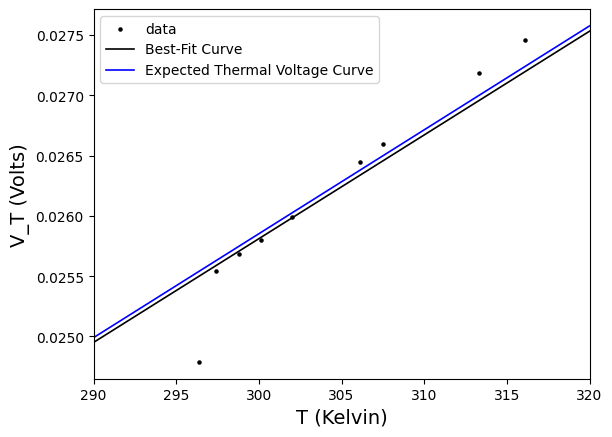
\includegraphics[width = .5\textwidth]{2_6SiBoltz.png}
		\caption{Temperature vs Thermal Voltage graph. The data points collected are represented by the black dots, our best-fit slope is the solid black curve, and the expected slope of $\frac{k}{e}$ is the solid blue curve.}
	
\end{figure}

%This is the most important section of the report.
%Describe data analysis. Details! Perhaps include a figure and refer
%the reader to it! See Figure~\ref{fig:apparatus}. Maybe you will need
%to include a table. See Table~\ref{tab:events}.
%
%Describe calculations of the final results.
%Thoroughly address error analysis and discussion of measurement
%uncertainties. Remember: NO EXPERIMENTAL RESULT CAN BE QUOTED
%WITHOUT AN ERROR BAR! Do not forget about random or systematic
%uncertainties. Be sure to propagate errors correctly!
%Include a demonstrative graph when possible.
%See Figure~\ref{fig:results}.
%
%
%Make final assessment and interpretation after that.
%Discuss apparatus problems if any. Suggestions for
%lab setup or approach improvements are welcome!
%
%=====================================================
%============ Importing pictures  ====================
%=====================================================



%===========================================================================
%=========================== Table 1 =======================================
%===========================================================================
%
% Note: the position of the table does not always depend on its position here. See
% http://en.wikibooks.org/wiki/LaTeX/Tables
% for details.
%

%\begin {table}[h]
%{
%{%\footnotesize
%\begin {center}
%\begin {tabular} {c | c c  c | c | c c }
%\hline\hline
%Run 			&   ~~POT~~ 		&
%\multicolumn{2}{ | c } {Predicted}  &   \multicolumn{2}  {| c} {Selected} \\
%Period		& $(10^{20})$	&
%\multicolumn{2}{ | c } {(No oscillations)}  &   \multicolumn{2}  {| c} {(Far Detector)} \\
%			    &
%			& \multicolumn{1} {| c } {~~~Fully} & \multicolumn{1} { c } {~~~Partially}
%			& \multicolumn{1} {| c } {~~~Fully} & \multicolumn{1} { c } {~~~Partially} \\
%			
%\hline
%I			& 1.269		
%			& \multicolumn{1} {| r } {426 } & \multicolumn{1} { r } {375 }
%		     	& \multicolumn{1} {| r } {318 } & \multicolumn{1} { r } {357 } \\
%
%II		     	& 1.943
%			& \multicolumn{1} {| r } {639 } & \multicolumn{1} { r } {565 }
%		    	& \multicolumn{1} {| r } {511 } & \multicolumn{1} { r } {555 } \\
%
%\hline
%Total			& 7.246
%			& \multicolumn{1} {| r } {2,451 } & \multicolumn{1} { r } {2,206 }
%		     	& \multicolumn{1} {| r } {1,986 } & \multicolumn{1} { r } {2,017 } \\
%
%\hline% \hline
%\end {tabular}
%\end {center}
%}
%}
%\caption {\label{tab:events}
%Predicted and observed numbers of events classified in the Far Detector as fully and
%partially reconstructed charged current interactions shown for all running periods.
% }
%\end {table}


%=====================================================
%============ Section ================================
%=====================================================

\section{Results}

Clearly present the result of your analysis. Make sure
you include the uncertainties. No experimental result
can be quoted without an error attached to it.

Your results should be compared with predictions and other
measurements.


%=====================================================
%============ Section ================================

\section{Summary and conlcusions}

Summarize briefly the results of the experiment.
Acknowledge (i.e., thank for) contributions or help
of your partner(s) and or
others (TA, machine shop, software used, ...).

%=====================================================
%============ Bibliography  ==========================
%=====================================================

\begin{thebibliography}{9}

\bibitem{book} R. Feynman, {\it QED}, Ch.7.

\bibitem{article}	
R.Dalitz, Proc. Roy. Soc. (London) {\bf A64}, 667 (1951)

\end{thebibliography}

%=====================================================
%============ End ====================================
%=====================================================

\end{document}

%=====================================================
%============ End ====================================
%=====================================================
